\documentclass[a4paper,12pt]{article}
\usepackage[slovene]{babel}
\usepackage[utf8]{inputenc}
\usepackage{amsmath,amssymb}
\usepackage[margin=2cm]{geometry}
\usepackage{lmodern}
\usepackage{titlesec}
\usepackage{xcolor}
\usepackage{tikz}
\usepackage{hyperref}  
\usepackage{cleveref}
\usepackage{pgfplots}
\usepackage{booktabs}
\usepackage{array}
\pgfplotsset{compat=1.18}
\usepackage{etoolbox}

\newcounter{secitemcount}
\newcounter{totalitemcount}
\newcommand{\allresults}{}

\pretocmd{\section}{%
  \setcounter{secitemcount}{0}%
  \gdef\currentsectiontitle{}%
}{}{}

\pretocmd{\section}{\gdef\currentsectiontitle{#1}}{}{}

\pretocmd{\item}{%
  \stepcounter{secitemcount}%
  \stepcounter{totalitemcount}%
}{}{}

\AtEndEnvironment{enumerate}{%
  \gappto{\allresults}{%
    \resultentry{\currentsectiontitle}{\arabic{secitemcount}}%
  }%
}

\newcommand{\resultentry}[2]{%
  \subsection*{#1 (število nalog: #2)}%
}

%%%%%%%%%%%%%%%%%%%%%%%%%%%%%%%%%%%%%%%%%%%%%%%%%%%
\definecolor{mybrown}{RGB}{140, 90, 40}
\definecolor{col1}{RGB}{70,130,180}
\definecolor{col2}{RGB}{255,165,0}
\definecolor{col3}{RGB}{60,179,113}
\definecolor{col4}{RGB}{220,80,60}
\definecolor{col5}{RGB}{180,100,220}

\titleformat{\section}
  {\large\bfseries}
  {%
    \fcolorbox{mybrown}{white}{\rule{1.2ex}{1.2ex}}%
    \quad\thesection
  }
  {0.8em}
  {}

\titleformat{\subsection}
  {\bfseries}
  {%
    \fcolorbox{mybrown}{white}{\rule{0.9ex}{0.9ex}}%
    \quad\thesubsection
  }
  {0.8em}
  {}

\newcommand{\DocTitle}[1]{%
  \begin{center}
    {\rule{\textwidth}{0.1mm}\\[0.4cm]
    \LARGE
    \fcolorbox{mybrown}{gray!40}{\rule{1.4ex}{1.4ex}}
    \quad #1
    }
  \end{center}
  \vspace{1em}
}

\begin{document}

\pagestyle{fancy}
\lhead{}\chead{}\rhead{}

\begin{center}
\Huge {\textbf{Test – Odvod funkcije}}
\end{center}

% ===================== 1 =====================
\subsection{ Izračunaj odvod funkcije:}

a) $f(x)=5x^3-2x^2+7x-3$

b) $g(x)=\dfrac{5}{x^3}$

\vspace{1cm}

% ===================== 2 =====================
\subsection{ Izračunaj odvod v dani točki:}

a) $f(x)=x^3-3x^2+2x$, \quad $x_0=3$

b) $g(x)=\dfrac{3x+2}{x-2}$, \quad $x_0=4$

\vspace{1cm}

% ===================== 3 =====================
\subsection{ Določi enačbo tangente na graf funkcije v dani točki:}

a) $f(x)=x^2$, \quad $x_0=2$

b) $g(x)=\sqrt{x}$, \quad $x_0=9$

c) $h(x)=\dfrac{1}{x}$, \quad $x_0=2$

\vspace{1cm}

% ===================== 4 =====================
\subsection{Določi kot, ki ga tangenta na graf funkcije v dani točki oklepa z osjo $x$:}

a) $f(x)=\dfrac{5}{x}$, \quad $x_0=2$

b) $g(x)=\dfrac{1}{4}x^3$, \quad $x_0=3$

\vspace{1cm}

% ===================== 5 =====================
\subsection{Izračunaj kot med krivuljama v presečišču:}

a) $f(x)=x^2$, \quad $g(x)=x^2-4x$

b) $f(x)=x^2+2$, \quad $g(x)=-x^2+6$

\vspace{1cm}

% ===================== 6 =====================
\subsection{Statistika – ocene dijakov}

Spodaj so podane ocene 40 dijakov pri matematiki:

\vspace{0.3cm}
\begin{center}
\begin{tabular}{|*{10}{c|}}
\hline
2 & 4 & 3 & 5 & 2 & 3 & 4 & 4 & 1 & 3 \\
\hline
4 & 5 & 2 & 3 & 4 & 1 & 3 & 4 & 5 & 2 \\
\hline
3 & 4 & 4 & 2 & 5 & 3 & 4 & 2 & 3 & 4 \\
\hline
1 & 3 & 5 & 4 & 2 & 4 & 3 & 5 & 4 & 3 \\
\hline
\end{tabular}
\end{center}

\vspace{0.4cm}

\textbf{Naloge:}

\begin{enumerate}
  \item[a)] Uredi podatke v frekvenčno tabelo z relativnimi frekvencami:

  \vspace{0.3cm}
  \begin{center}
  \renewcommand{\arraystretch}{1.6}
  \begin{tabular}{|c|c|c|c|}
  \hline
  \textbf{Ocena} & \textbf{Frekvenca} $f_i$ & \textbf{Rel. frekvenca} $f_i / n$ & \textbf{Rel. frekvenca [\%]} \\
  \hline
  1 & & & \\
  \hline
  2 & & & \\
  \hline
  3 & & & \\
  \hline
  4 & & & \\
  \hline
  5 & & & \\
  \hline
  \textbf{Skupaj} & \textbf{40} & \textbf{1} & \textbf{100\%} \\
  \hline
  \end{tabular}
  \end{center}

  \vspace{0.5cm}

  \item[b)] Izračunaj \textbf{modus}, \textbf{mediano} in \textbf{aritmetično sredino}.

  \vspace{3cm}

  \item[c)] Prikaži porazdelitev ocen s \textbf{krožnim diagramom}. Označi vsak izsek z oceno in odstotkom.

  \vspace{5cm}

\end{enumerate}

\vfill

\newpage

% ===================== REŠITVE =====================
\section*{Rešitve}

\subsection*{1}
a)
\[
f'(x)=15x^2-4x+7
\]

b)
\[
g(x)=5x^{-3} \Rightarrow g'(x)=-15x^{-4}=-\frac{15}{x^4}
\]

\subsection*{2}
a)
\[
f'(x)=3x^2-6x+2, \quad f'(3)=27-18+2=11
\]

b)
\[
g'(x)=\frac{3(x-2)-(3x+2)}{(x-2)^2}=\frac{-8}{(x-2)^2}, \quad g'(4)=\frac{-8}{4}=-2
\]

\subsection*{3}
Uporabimo: $y=f'(x_0)(x-x_0)+f(x_0)$

a)
\[
f'(x)=2x,\quad f'(2)=4,\quad f(2)=4 \quad\Rightarrow\quad y=4x-4
\]

b)
\[
g'(x)=\frac{1}{2\sqrt{x}},\quad g'(9)=\frac{1}{6},\quad g(9)=3 \quad\Rightarrow\quad y=\frac{1}{6}(x-9)+3
\]

c)
\[
h'(x)=-\frac{1}{x^2},\quad h'(2)=-\frac{1}{4},\quad h(2)=\frac{1}{2} \quad\Rightarrow\quad y=-\frac{1}{4}x+1
\]

\subsection*{4}
Velja: $\tan \alpha = f'(x_0)$

a)
\[
f'(x)=-\frac{5}{x^2},\quad f'(2)=-\frac{5}{4} \quad\Rightarrow\quad \alpha=\arctan\!\left(-\tfrac{5}{4}\right)
\]

b)
\[
g'(x)=\frac{3}{4}x^2,\quad g'(3)=\frac{27}{4} \quad\Rightarrow\quad \alpha=\arctan\!\left(\tfrac{27}{4}\right)
\]

\subsection*{5}
Formula: $\tan \varphi = \left|\dfrac{k_1-k_2}{1+k_1k_2}\right|$

a) Presečišče: $x^2=x^2-4x \Rightarrow x=0$
\[
k_1=0,\quad k_2=-4 \quad\Rightarrow\quad \tan \varphi = 4
\]

b) Presečišče: $x^2+2=-x^2+6 \Rightarrow x=\pm\sqrt{2}$

Za $x=\sqrt{2}$:
\[
k_1=2\sqrt{2},\quad k_2=-2\sqrt{2} \quad\Rightarrow\quad
\tan \varphi = \left|\frac{4\sqrt{2}}{1-8}\right|=\frac{4\sqrt{2}}{7}
\]

\subsection*{6}

\textbf{a) Frekvenčna tabela:}

\vspace{0.3cm}
\begin{center}
\renewcommand{\arraystretch}{1.5}
\begin{tabular}{|c|c|c|c|}
\hline
\textbf{Ocena} & \textbf{Frekvenca} $f_i$ & \textbf{Rel. frekvenca} $f_i/n$ & \textbf{Rel. frekvenca [\%]} \\
\hline
1 & 3  & 0{,}075 & 7{,}5\% \\
\hline
2 & 7  & 0{,}175 & 17{,}5\% \\
\hline
3 & 11 & 0{,}275 & 27{,}5\% \\
\hline
4 & 13 & 0{,}325 & 32{,}5\% \\
\hline
5 & 6  & 0{,}150 & 15{,}0\% \\
\hline
\textbf{Skupaj} & \textbf{40} & \textbf{1} & \textbf{100\%} \\
\hline
\end{tabular}
\end{center}

\vspace{0.5cm}

\textbf{b) Mere srednje vrednosti:}

\textbf{Modus} (najpogostejša vrednost):
\[
Mo = 4 \quad \text{(frekvenca 13)}
\]

\textbf{Mediana} (srednja vrednost urejenega niza, $n=40$):

Urejen niz: 3 ocene 1, 7 ocen 2, 11 ocen 3, 13 ocen 4, 6 ocen 5.

20. in 21. vrednost sta obe enaki 4 (saj do ocene 3 pridemo pri 21. elementu):
\[
Me = \frac{x_{20}+x_{21}}{2} = \frac{3+4}{2} = 3{,}5
\]

\textbf{Aritmetična sredina}:
\[
\bar{x} = \frac{\sum f_i \cdot x_i}{n}
= \frac{3\cdot1 + 7\cdot2 + 11\cdot3 + 13\cdot4 + 6\cdot5}{40}
= \frac{3+14+33+52+30}{40}
= \frac{132}{40} = 3{,}3
\]

\vspace{0.5cm}

\textbf{c) Krožni diagram:}

\vspace{0.3cm}
\begin{center}
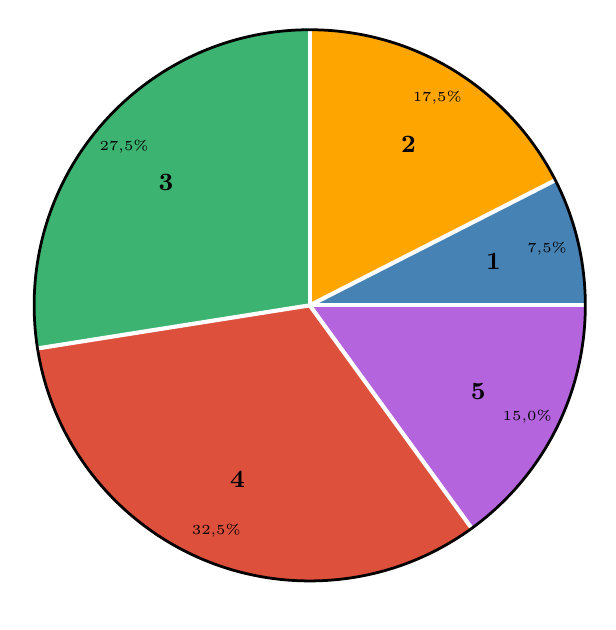
\begin{tikzpicture}
  % koti: ocena 1 = 7.5% = 27°, 2 = 17.5% = 63°, 3 = 27.5% = 99°, 4 = 32.5% = 117°, 5 = 15% = 54°
  \def\r{3.5}
  % ocena 1: 0° do 27°
  \fill[col1]   (0,0) -- ({cos(0)*\r},{sin(0)*\r})
    arc[start angle=0, end angle=27, radius=\r] -- cycle;
  % ocena 2: 27° do 90°
  \fill[col2]   (0,0) -- ({cos(27)*\r},{sin(27)*\r})
    arc[start angle=27, end angle=90, radius=\r] -- cycle;
  % ocena 3: 90° do 189°
  \fill[col3]   (0,0) -- ({cos(90)*\r},{sin(90)*\r})
    arc[start angle=90, end angle=189, radius=\r] -- cycle;
  % ocena 4: 189° do 306°
  \fill[col4]   (0,0) -- ({cos(189)*\r},{sin(189)*\r})
    arc[start angle=189, end angle=306, radius=\r] -- cycle;
  % ocena 5: 306° do 360°
  \fill[col5]   (0,0) -- ({cos(306)*\r},{sin(306)*\r})
    arc[start angle=306, end angle=360, radius=\r] -- cycle;

  % robovi
  \draw[white, line width=1.5pt] (0,0) -- ({cos(0)*\r},{sin(0)*\r});
  \draw[white, line width=1.5pt] (0,0) -- ({cos(27)*\r},{sin(27)*\r});
  \draw[white, line width=1.5pt] (0,0) -- ({cos(90)*\r},{sin(90)*\r});
  \draw[white, line width=1.5pt] (0,0) -- ({cos(189)*\r},{sin(189)*\r});
  \draw[white, line width=1.5pt] (0,0) -- ({cos(306)*\r},{sin(306)*\r});
  \draw[black, line width=1pt] (0,0) circle (\r);

  % oznake
  \node at ({cos(13.5)*2.4},{sin(13.5)*2.4})  {\small\textbf{1}};
  \node at ({cos(13.5)*3.1},{sin(13.5)*3.1})  {\tiny 7{,}5\%};

  \node at ({cos(58.5)*2.4},{sin(58.5)*2.4})  {\small\textbf{2}};
  \node at ({cos(58.5)*3.1},{sin(58.5)*3.1})  {\tiny 17{,}5\%};

  \node at ({cos(139.5)*2.4},{sin(139.5)*2.4}) {\small\textbf{3}};
  \node at ({cos(139.5)*3.1},{sin(139.5)*3.1}) {\tiny 27{,}5\%};

  \node at ({cos(247.5)*2.4},{sin(247.5)*2.4}) {\small\textbf{4}};
  \node at ({cos(247.5)*3.1},{sin(247.5)*3.1}) {\tiny 32{,}5\%};

  \node at ({cos(333)*2.4},{sin(333)*2.4})    {\small\textbf{5}};
  \node at ({cos(333)*3.1},{sin(333)*3.1})    {\tiny 15{,}0\%};

\end{tikzpicture}

\vspace{0.4cm}
% Legenda
\begin{tikzpicture}
  \foreach \i/\col/\lbl in {
    0/col1/Ocena 1 (7{,}5\%),
    1/col2/Ocena 2 (17{,}5\%),
    2/col3/Ocena 3 (27{,}5\%),
    3/col4/Ocena 4 (32{,}5\%),
    4/col5/Ocena 5 (15{,}0\%)} {
      \fill[\col] ({2.8*\i}-5.6, 0) rectangle ({2.8*\i}-5.6+0.4, 0.4);
      \node[anchor=west] at ({2.8*\i}-5.2, 0.2) {\small\lbl};
  }
\end{tikzpicture}
\end{center}

\end{document}
